\section{NSCs}

Im folgenden die wichtigsten Charaktere mit denen es die Spieler zu tun bekommen aufgeteilt nach Ort des Geschehens.

\subsection{Cowboybrigade}

Die Cowboybrigade sind 5 Alphas, Spezialisten f"ur Raumschifftechnik, Arbeit mit Exoskelett im Luftlehren Raum, Drohneneinsatz.
Angestellt bis vor 6 Wochen am Raumhafen von Valhalla auf Callisto. Dann ausgeliehen an die Protektoratsgarnison am Raumhafen von Valhalla und vor ca.~4 Wochen ausgeliehen an Armageddon. Die Cowboybrigade stammt urspr"nglich aus dem Asteroideng"urtel G"urtel zwischen Mars und Jupiter und ist vor wahrscheinlich einem Jahr auf Callisto.

\begin{itemize}
    \item Stetson: Der Anf"uhrer, gro\3 und dratig.
    \item Quckfinger Rod: Vorlaut, immer ein Kartenspiel in der Hand.
    \item Joe Rider: Klein, gedrungen, spricht nicht wenn nicht unbedingt n"otig.
    \item Tom Gunslinger: Der Vern"unftige.
    \item Slingshot (Drake): Das ``Nesth"akchen'' der Gruppe. Drake ist der Name unter dem er in nach dem Attentat auf Armageddon auf Hellgate auftaucht.
\end{itemize}

Slingshot ist einer der Attent"ater, ein Alpha dessen Gehirn durch eine von der USI kontrollierten KI "ubernommen wurde.
Auf Hellgate tritt er nach dem Vorfall auf Armageddon unter dem Namen Drake auf.

\textbf{Slingshot: Fight +4, Agility +4, Body +2, HP 10}

\newpage

\subsection{Pers"onlichkeiten auf Hellgate}

Auf Hellgate gibt es folgende Pers"onlichkeiten:

\begin{itemize}
    \item Dr.~Acra Link: Technische Leitung der Hellgate Station
    \item Sina Hendrik: Administrative Leitung der Hellgate Station
    \item Dr.~Petrova: Technische Leitung der F"orderminen
    \item Henk Arongate: Sicherheitschef    
    \item Kriegsmeister Jos\'{e} \frqq{}Toro\flqq{} Alvarez: Norm. Ausbilder der Jagdverb"ande des Protektorats, Kriegsheld.
\end{itemize}

\subsection{Sicherheitspersonal Hellgate}

Neben \emph{Grace Enders} sind folgende Personen des Sicherheitsdienstes relevant:

\begin{itemize}
    \item Henk Arongate: Sicherheitschef    
    \item Karl Sanders: Stationsleiter des St"utzpunkts der Sicherheitskr"afte. Vorgesetzter von Grace Anders.
    \item Luke Dexter: Trupp F"uhrer der Sondereinsatzgruppe f"ur die Befreiung der Geiseln.
    \item Lionel Flin: Mitarbeiter Sicherheitsdienst. Wird bei der Geiselname auf dem Sicherheitsst"utzpunkt schwer verletzt. Ehemaliger Freund von Grace Enders.
\end{itemize}

\subsection{Grace Anders}

Grace Anders ist eine Mitarbeiterin des Sicherheitsdienstes auf Hellgate. Sie wird von Chef Henk Arongate zur Unterst"utung der Charaktere abgestellt. Grace Anders ist Mitte 30 ist h"ubsch mit kurzen blonden Haaren. W"ahrend der Unterst"utzung der Charaktere tr"agt sie die Schutzkleidung des Sicherheitsdienstes mit schu\3sicherer Weste, Schlagstock, Handschellen und einer Schu\3waffe. Gace Anders stamt urspr§unglich vom Mars und hat sich ins Jovianische System auf der Suche nach neuen Herausforderungen versetzen lassen. Sie war mit Luke Lengdon der Sicherheitsmann bei der folgenden Geiselname schwer verletzt wurde liiert hat sich aber vor kurzem von ihm getrennt.

Grace Anders begleitet die Charaketere w"ahrend des aufenthalts auf Hellgate und berichtet regelm"aßig an \emph{Karl Sanders} ihren vorgesetzten. "Uber Grace Anders k"onnen sie Informationen bzgl.~der Minen und Personal der Station und der Mienen anfragen. W"ahrend der Entf"uhrung kann sie die Charaktere unterst"uten.

\subsection{Besatzung HeM05}

Folgende Personen waren w"ahrend des Attentats auf HeM05:

\begin{itemize}
    \item Florence: Beta Mutant, Kommandant der Mine
    \item ZDee: Alpha Mutant Minenarbeiter (tot)
    \item Greydog: Alpha Mutant, Minenarbeiter
    \item Isabell Sonderleiten: Norm, Chemikerin, Stellvertreterin von Florence
    \item Juri Smirnov: Norm, Logistik
    \item Fernandez Lorend: Norm, Techniker
    \item Hanibal: Alpha Mutant, Techniker der Minensteueranlage, Attent"ater
    \item Pitch: Alpha Mutant, Technikerin der HE-3 der Minensteueranlage
    \item Salvador: Norm, Physiker, Weltraumtechnik
    \item Blackwind: Beta, Sicherheitsdienst
\end{itemize}

All Mitarbeiter auf der Mine au\3er Fernand, Salvador, Greydog und Pitch waren vor dem Jupitereinsatz bereits im Dienst der Cynarion Corporation.

\subsection[\pinyin{Wang Xiao Long}]{\pinyin{Wang2} \pinyin{Xiao3} \pinyin{Long2}}

\pinyin{Wang2} \pinyin{Xiao3} \pinyin{Long2} entstammt einer reichen Familie aus den F"uhrungsreihen der USI Corporation. Fr"uhzeitig hat sie sich von ihrer Familie abgewandt und ist zu einer der ber"ucktigsten Pirantenf"uhrer des Asteroideng"urtel geworden. 

\begin{wrapfigure}{r}
    {0.55\textwidth}\fbox{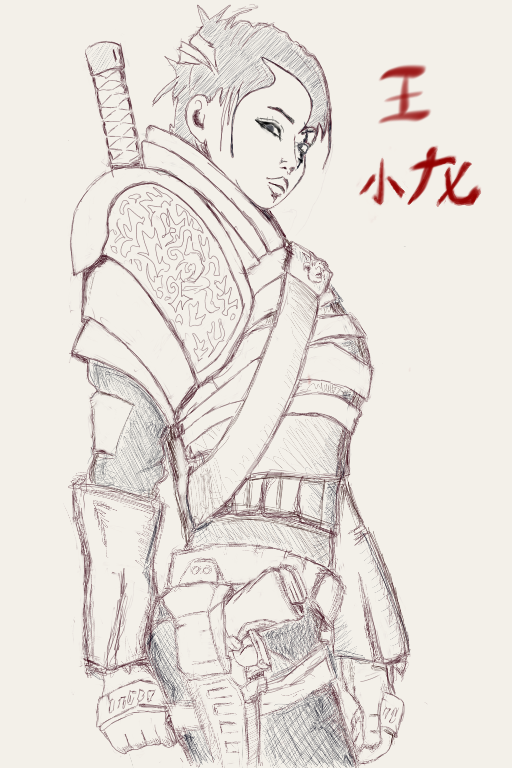
\includegraphics[width=0.9\linewidth]{./images/wang_xiao_long.png}}
    \caption{\pinyin{Wang2} \pinyin{Xiao3} \pinyin{Long2}}
\end{wrapfigure}

Nach ihrer Gefangennahme wurde sie vor 2 Jahren zum Hochsicherheitsgef"angnis Blackpit auf Vahlhalla verlegt. Dort machte man ihr das Angebot einer Haftentlassung im Gegenzug zur Teilnahme an einem klinischen Experiment.

Beim durchgef"uhrten klinischen Experiment handelt es sich um das Einsetzen einer der von Dr.~Naratova entwickelten ``freien KI'' Symbionten. Die Oeration wurde durch Prof.~Dr.~Sanders durchgef"uhrt. Prof.~Dr.~Sanders handelte dabei im direkten Auftrag von Dr.~Naratovas ohne das Wissen der USI Agenten Smith-Singer und Frederic Johnson. Durch ihre starke Pers"onlichkeit konnte \pinyin{Xiao3} \pinyin{Long2} verhindern da\3 die KI ihren Geist vollst"andig "ubernehmen konnte und so verschmolzen der Geist und das artifizielle Gehirnzu einer Symbiose genau so wie Dr.~Naratova es sich immer erhofft hatte.

Nach ihrer Haftentlassung schlo\3 sich \pinyin{Xiao3} \pinyin{Long2} dem Luna--Syndikats an und stieg dort schnell zu einem der Capos der Organisation. Duke Nemessis wei\3 um ihre Vergangenheit. Die Verwandlung in eine KI ist ihm allerdings nicht bekannt. Ihm ist Sie als geflohene Verrecherin bekannt.

\pinyin{Xiao3} \pinyin{Long2} ist eine hochgewachsene Asiatin, ein Pure, die sich gerne als Samurai mit entsprechender R"usting gibt. Sie ist intelligent, gewitzt, skrupellos und liebt das Risiko. Durch ihre finanziellen M"oglichkeiten und Kontakte in ihrem fr"uheren Leben hat Sie ihren K"orper durch zahllose Modifikationen zu einer Kampfmaschiene entwickelt die einem Omega in nichts nachsteht was f"ur einen Norm sehr ungew"ohnlich ist.

Im Rahmen der Geschichte verfolgt sie das Ziel die Forschungsergebnisse Naratovas an sich zu bringen und alle Informationen zu den freien KIs wie auch das Wissen "uber die Technologie zu vernichten. Daf"ur wird sie alle an den Experimenten beteiligten Personen Naratova, Sanders, die USI Agenten und deren Wissenschaftler t"oten und Forschungseinrichtungen zerst"oren solange sie dabei den Verdacht nicht auf sich lenkt. An der Identit"at der anderen KIs ist sie nicht interessiert.

Vor dem Zusammentreffen mit den Charakteren kennt sie den Standort und den Namen der USI Tochter Cyberbrain nicht.

\pinyin{Wang2} \pinyin{Xiao3} \pinyin{Long2}: Fight +9, Agility +10, Body +4, HP 14
